\section{Definition (Fabi)}
\label{definition-fabi}

\begin{figure}[h]
	\centering
	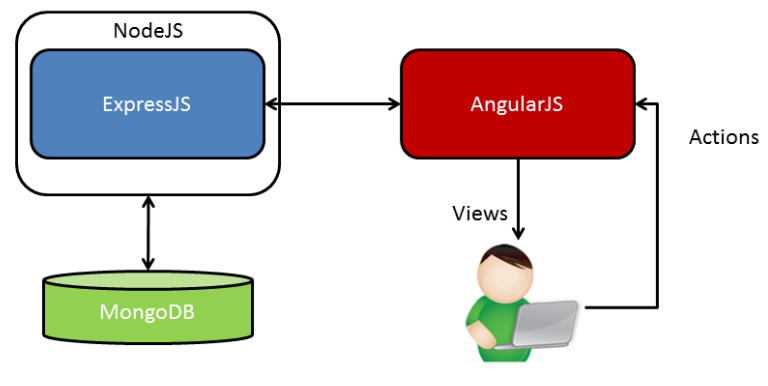
\includegraphics[width=0.7\linewidth]{figures/mean-grobarchitektur.png}
	\caption{MEAN Grobarchitektur}
	\label{f:mean-grobarchitektur}
\end{figure}

Zuerst ist zu sagen, dass es sich bei MEAN nicht um einen fest definierten Stack handelt. MEAN bedeutet lediglich, dass die MongoDB, Express, AngularJS und NodeJS Technologien zum Einsatz kommen. Damit soll das MEAN Konzept den LAMP Stack ersetzen. Wenn man sich mit der MEAN Thematik beschäftigt stößt man daher auch auf mehrere unterschiedliche MEAN Stacks, unter anderem z.B. MEAN.IO oder MEAN.JS.

In der Abbildung \ref{f:mean-grobarchitektur} sind die groben Zusammenhänge der Frameworks ersichtlich.

Bei MongoDB handelt es sich um die populärste NoSQL Datenbank, die vor allem für ihre Skalierbarkeit bekannt ist. Als Webframework für Node kommt Express zum Einsatz. AngularJS wird im Frontend zur Entwicklung von Single-page-Webanwendungen nach dem MVC-Pattern eingesetzt. Erwähnenswert hierbei ist das AngularJS von Google entwickelt wurde. Zu guter letzt wird das verbreitete Node Framework im Backend Bereich verwendet.